% Created 2016-04-06 ons 13:25
% Intended LaTeX compiler: pdflatex
\documentclass{scrartcl}
\usepackage[utf8]{inputenc}
\usepackage[T1]{fontenc}
\usepackage{graphicx}
\usepackage{grffile}
\usepackage{longtable}
\usepackage{wrapfig}
\usepackage{rotating}
\usepackage[normalem]{ulem}
\usepackage{amsmath}
\usepackage{textcomp}
\usepackage{amssymb}
\usepackage{capt-of}
\usepackage{hyperref}
\usepackage{khpreamble}
\author{Kjartan Halvorsen}
\date{Due 2016-03-21}
\title{Computerized control - homework 3}
\hypersetup{
 pdfauthor={Kjartan Halvorsen},
 pdftitle={Computerized control - homework 3},
 pdfkeywords={},
 pdfsubject={},
 pdfcreator={Emacs 24.5.1 (Org mode 8.3.4)}, 
 pdflang={English}}
\begin{document}

\maketitle

\section*{The system}
\label{sec:orgheadline1}
A feedback system for level control of a tank is shown in the figure below.
\begin{center}
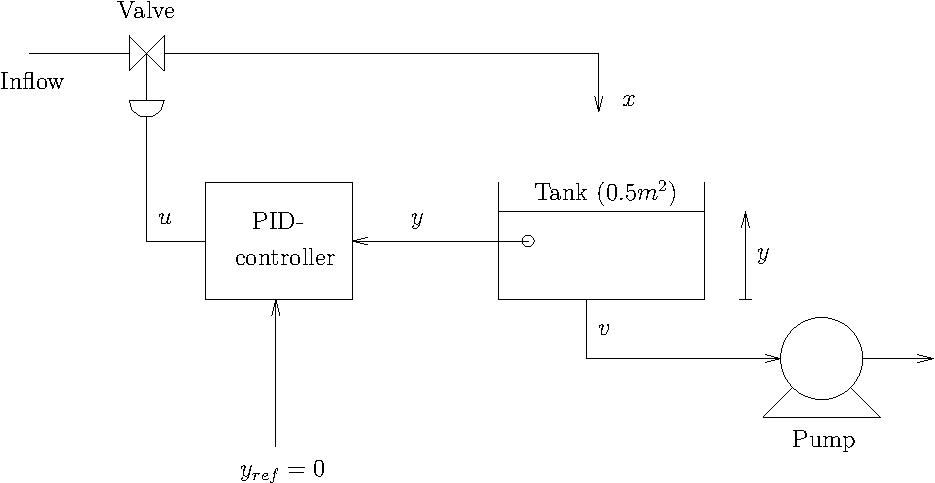
\includegraphics[width=\linewidth]{tank-system-crop}
\caption{Feedback system for level control. Alla variables are variations from a working point. Water is pumped from the water tank as needed by some industrial process downstream.}
\end{center}
The flow of water, \(x(t)\) does not change immediately with a change of input \(u(t)\) to the valve, but reacts as a first order system
\[ \frac{dx}{dt} = -2x + 4u. \]
The flows \(x(t)\) and \(v(t)\) has the dimension \unit{}{\meter\cubed\per\second}.

The PID controller has transfer function 
\[ F(s) = K_P + sK_D + \frac{K_I}{s}. \]

\section*{Exercises}
\label{sec:orgheadline7}
\subsection*{Problem 1}
\label{sec:orgheadline2}
Draw a block diagram of the system, and derive the transfer function for the closed-loop system
\[ Y(s) = G_c(s)Y_{ref}(s) - S(s)V(s) = \frac{G_1(s)G_2(s)F(s)}{1 + G_1(s)G_2(s)F(s)} Y_{ref}(s) - \frac{G_1(s)}{1 + G_1(s)G_2(s)F(s)}V(s), \]
where
\begin{align}
G_1(s) &= \frac{2}{s}\\
G_2(s) &= \frac{4}{s+2}.
\end{align}

\subsection*{Problem 2}
\label{sec:orgheadline3}
Show that the transfer function from the outlet \(-v(t)\) to the variation in the water level \(y(t)\) is given by 
\[ S(s) = \frac{2s(s+2)}{s^3 + (2+8K_D)s^2  + 8K_Ps + 8K_I}. \]

\subsection*{Problem 3}
\label{sec:orgheadline4}
Consider the three different settings of the PID-controller in the table below. Pair each of the settings with the correct pole-zero plot of \(S(s)\) and the correct response of the water level to a step in \(v(t)\). 

\begin{center}
\begin{tabular}{lrrr}
 & \(K_P\) & \(K_I\) & \(K_D\)\\
\hline
I & 2 & 0 & 0\\
\hline
II & 4 & 1 & 0\\
\hline
III & 2 & 2 & 1\\
\hline
\end{tabular}
\end{center}

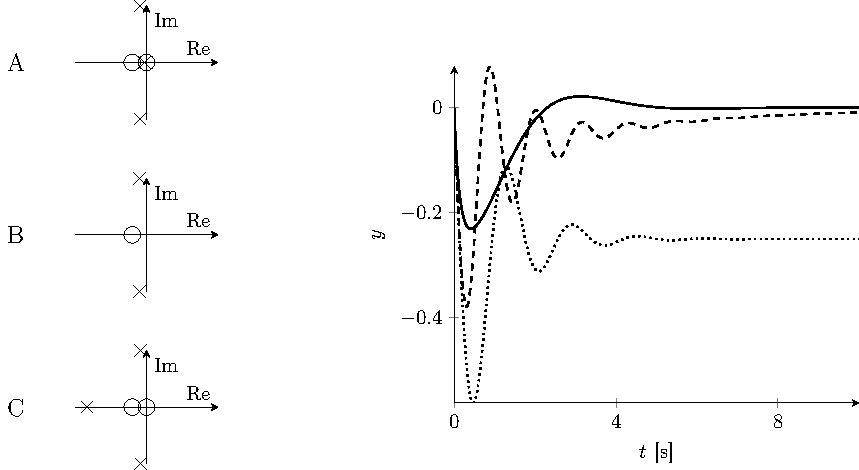
\includegraphics[width=\linewidth]{tank-system-step-response}

\subsection*{Problem 4}
\label{sec:orgheadline5}
Assume that there is a small delay of \(T_d=\unit{0.1}{\second}\) in the feedback path of the controller. Tune the PID controller using the Ziegler-Nicholls ultimate sensitivity method (Table 8.3 in Å\&W). To do this, you need to implement the feedback system in matlab using a P-controller. Do step-responses, and crank up the gain of the P-controller until you get sustained oscillations. The corresponding gain is the so-called \emph{ultimate gain} \(K_u\). Find the period of the oscillations, \(T_u\), at this gain. From these two values you can determine the PID controller parameters from Table 8.3.

Here is some matlab code to get you started
\begin{verbatim}
% The plant model
Td = 0.1;
s = tf('s');
G1 = 2/s;
G2 = 4/(s+2);
G = G1*G2

% Set D and I gain to zero and try different values of the proportional 
% gain of the controller
Ki = 0;
Kd = 0;
Kp = 2
F = Kp + s*Kd + Ki/s;

% The loop gain and closed loop system
Go = G*F;
Gc = feedback(Go,exp(-Td*s)); % Note the delay in the feedback path

% Step response
figure(1)
clf
step(Gc, 10)
\end{verbatim}

\textbf{Include a step response with the PID parameters you found!}

\subsection*{Problem 5}
\label{sec:orgheadline6}
\begin{enumerate}
\item Discretize your PID controller for general sampling period \(h\) using Tustin's formula.
\item Simulate the discretized model in matlab using a sampling period that is equal to the time delay \(T_d\). Here is some code to help:
\begin{verbatim}
Gd = c2d(G, Td, 'zoh'); % Discretize plant model to be able to simulate
Fd = c2d(F, Td, 'tustin')
God = Gd*Fd;
Gcd = feedback(God,tf([1],[1 0], Td)); % Note the delay in the feedback path

% Step response
figure(1)
clf
step(Gc, Gcd, 10)
\end{verbatim}
\textbf{Include the step response in your report.}
\item Discuss in 2-4 sentences the difference between the response using the continuous PID controller and the discretized PID controller.
\end{enumerate}
\section*{Solutions}
\label{sec:orgheadline16}
\subsection*{Problem 1}
\label{sec:orgheadline8}
\begin{tikzpicture}[node distance=2.6cm, block/.style={rectangle, draw, minimum height=15mm, minimum width=20mm}, sumnode/.style={circle, draw, inner sep=1pt}]

  \node[coordinate] (input) {};
  \node[sumnode, right of=input] (sum) {$\sum$};
  \node[block, right of=sum] (control) {PID};
  \node[block, right of=control, node distance=3.1cm] (valve) {$G_2$};
  \node[sumnode, right of=valve] (sumdist) {$\sum$};
  \node[block, right of=sumdist] (tank) {$G_1$};
  \node[coordinate, right of=tank] (output) {};
  \draw[->] (tank) -- node[coordinate] (measure) {} node[above, pos=0.9] {$y$} (output);

  \node[coordinate, above of=sumdist, node distance=2cm] (dist) {};

  \draw[->] (input) -- node[above, pos=0.2] {$y_{ref}$} (sum);
  \draw[->] (sum) -- node[above] {$e$} (control);
  \draw[->] (control) -- node[above] {$u$} (valve);
  \draw[->] (valve) -- node[above] {$x$} (sumdist);
  \draw[->] (dist) -- node[left]{$v$} node[right, pos=0.9] {$-$} (sumdist);
  \draw[->] (sumdist)  to (tank);
  \draw[->] (measure) |- ++(-2cm, -2cm) -| node[pos=0.97, right] {$-$} (sum);
\end{tikzpicture}

Transform the signals to the Laplace-domain and write the PID controller as the transfer function \(F(s)\). 
\begin{equation*}
 \begin{split}
  Y &= G_1(X-V) = G_1(G_2FE-V) = G_1\big(G_2F(Y_{ref}-Y)-V\big)\\
  (I + G_1G_2F) Y &= G_1G_2FY_{ref} - G_1V\\
   Y &= \underbrace{\frac{G_1G_2F}{1 + G_1G_2F}}_{G_c(s)} Y_{ref} - \underbrace{\frac{G_1}{1 + G_1G_2F}}_{S(s)}V
 \end{split}
\end{equation*}
\subsection*{Problem 2}
\label{sec:orgheadline9}
Substituting \(F(s) = K_P + sK_D + K_I/s\), \(G_1(s)= 2/s\) and \(G_2(s) = 4/(s+2)\) into the expression for \(S(s)\) gives
\begin{equation*}
 \begin{split}
 S(s) &= \frac{2/s}{1 + \frac{2}{s}\frac{4}{s+2}(K_P + sK_D + K_I/s)}\\
      &= \frac{2(s+2)}{s(s+2) + 8(K_P + sK_D + K_I/s)}\\
      &= \frac{2s(s+2)}{s^2(s+2) + 8K_Ds^2 + 8K_Ps + 8K_I}\\
      &= \frac{2s(s+2)}{s^3 + (2 + 8K_D)s^2 + 8K_Ps + 8K_I}
 \end{split}
\end{equation*}

\subsection*{Problem 3}
\label{sec:orgheadline13}
\subsubsection*{Setting I - P control}
\label{sec:orgheadline10}
Setting I is pure proportional control, so \(K_D=K_I=0\). This gives
\[ S(s) = \frac{2s(s+2)}{s^3 + 2s^2 + 8K_Ps} = \frac{2(s+2)}{s^2 + 2s + 16} \]
with one zero at \(s=-2\) and two complex-conjugated poles in \(s = -1 \pm 3.873i\). This must correspond to the zero-pole plot \textbf{B}. The step response will have a stationary error, since there is no zero in the origin. This corresponds to the \textbf{dotted line}.
\subsubsection*{Setting II - PI control}
\label{sec:orgheadline11}
Setting II gives the transfer function
\[ S(s) = \frac{2s(s+2)}{s^3 + 2s^2 + 8K_Ps + 8K_I} = \frac{2s(s+2)}{s^3 + 2s^2 + 32s + 8}\]
with zeros at -2 and in the origin and poles in \(s=-0.2535\) and \(s = -0.8732 \pm 5.549i\). This must correspond to the zero-pole plot \textbf{A}. The PI controller has higher gain compared to the P controller with setting I, and an integrating term, which gives the two fast poles with small damping. We also have a dominating pole close to the origin, which gives a slow response. Hence, the corresponding step-response must be the \textbf{dashed line}.
\subsubsection*{Setting III - PID control}
\label{sec:orgheadline12}
By elimination, we now have that this corresponds to zero-pole plot \textbf{C} and the \textbf{solid line} in the step-response. This can also be seen by calculating the poles of the transfer function
\[ S(s) = \frac{2s(s+2)}{s^3 + 10s^2 + 16s + 16}.\]
The poles are \(s=-8.3055\) and \(s = -0.8472 \pm 1.0994i\). The response has reasonable damping.
\subsection*{Problem 4}
\label{sec:orgheadline14}
Trying a few different values for \(K_P\) leads to \(K_u = 2.58\). A step-response of the closed-loop system with this ultimate gain is shown below
\begin{center}
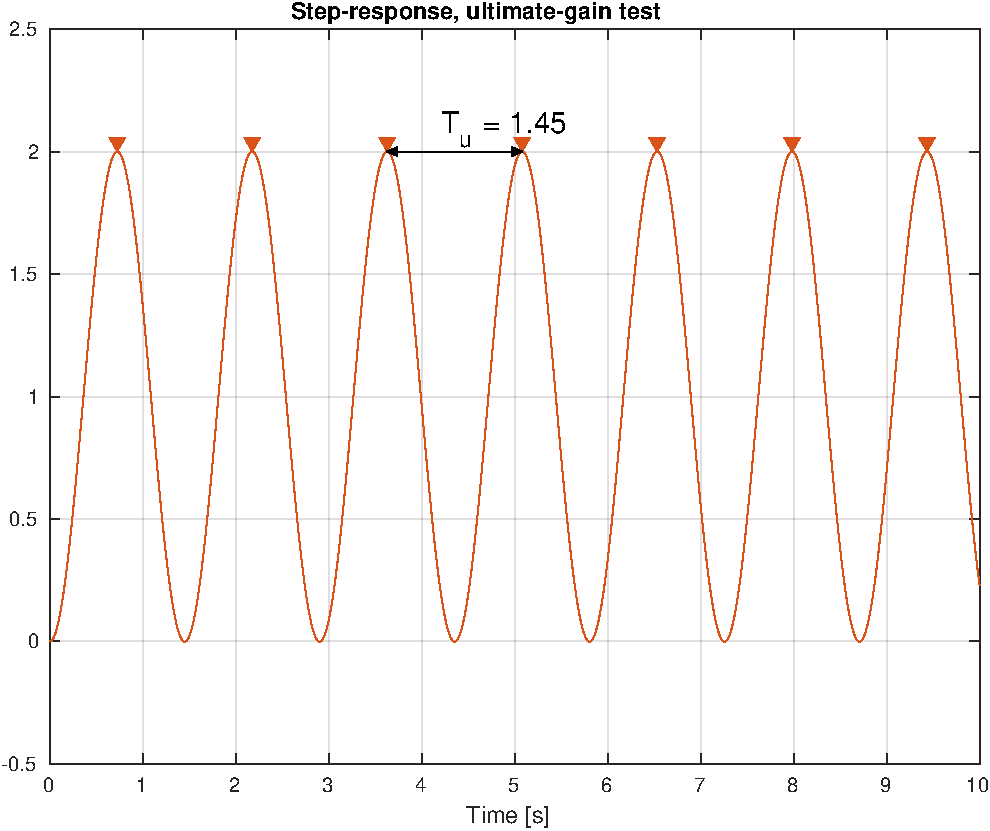
\includegraphics[width=0.6\linewidth]{ultimate_period_hw3_spring16}
\end{center}

Using table 8.3 in Å\&W, we get the PID controller
\[F(s) = K(1 + \frac{1}{T_is} + T_ds) = 0.6K_u(1 + \frac{1}{0.5T_us} + 0.125T_us) = 1.548\big(1 + \frac{1}{0.725s} +  0.1812 s\big). \]

The step response of the closed-loop system (also with discretized controller) is shown below.
\begin{center}
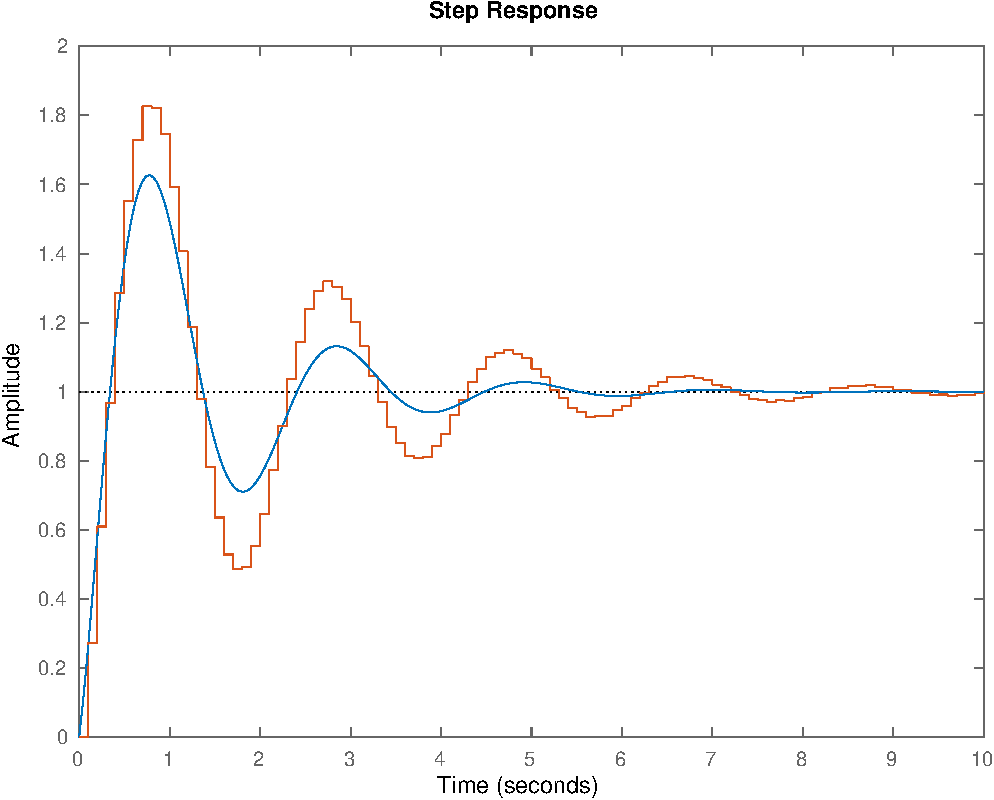
\includegraphics[width=0.6\linewidth]{tuned_response_hw3_spring16}
\end{center}

\subsection*{Problem 5}
\label{sec:orgheadline15}
\begin{enumerate}
\item Discretizing the controller using Tustin's approximation gives
\begin{equation*}
\begin{split}
 F_d(z) &= F(s)|_{s=\frac{2}{h}\frac{z-1}{z+1}}\\
       &= 1.548 \frac{0.1812s^2 + s +1/0.725}{s}|_{s=\frac{2}{h}\frac{z-1}{z+1}}\\
       &= 1.548 \frac{0.1812 \left( \frac{2}{h}\frac{z-1}{z+1} \right)^2 + \frac{2}{h}\frac{z-1}{z+1} + 1.3793}{\frac{2}{h}\frac{z-1}{z+1}}\\  
       &= 1.548 \frac{0.1812 \frac{4(z-1)^2}{h(z+1)} + 2(z-1) + 1.3793 h(z+1)}{2(z-1)}\\
       &= 1.548 \frac{0.7248 (z-1)^2 + 2h(z-1)(z+1) + 1.3793 h^2(z+1)^2}{2h(z-1)(z+1)}\\
       \end{split}
\end{equation*}
\item Discretizing the controller and doing a step-response test gives the figure already shown above under Problem 4.
\item The discretized controller gives a system with less damping. The discretization involves a sample-and-hold, which gives a time-delay of approximately \(h/2\). This explains the smaller damping. The discretization of the controller is an approximation, so we cannot expect better performance with the discrete controller, but as the sampling period dicreases, the performance will be closer to that of the contninuous controller. This is illustrated in the figure below. 
\begin{center}
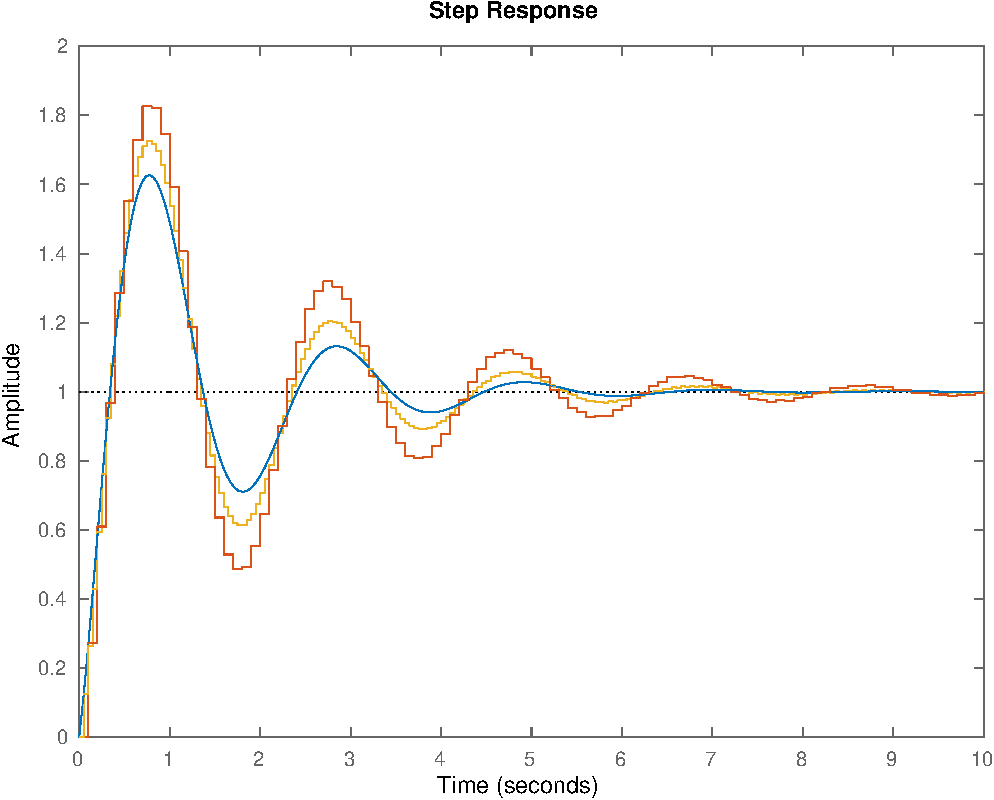
\includegraphics[width=0.6\linewidth]{tuned_response_half_h_hw3_spring16}
\end{center}
\end{enumerate}
\end{document}
